\documentclass{standalone}
\usepackage{tikz}
\usetikzlibrary{patterns, positioning}

\begin{document}
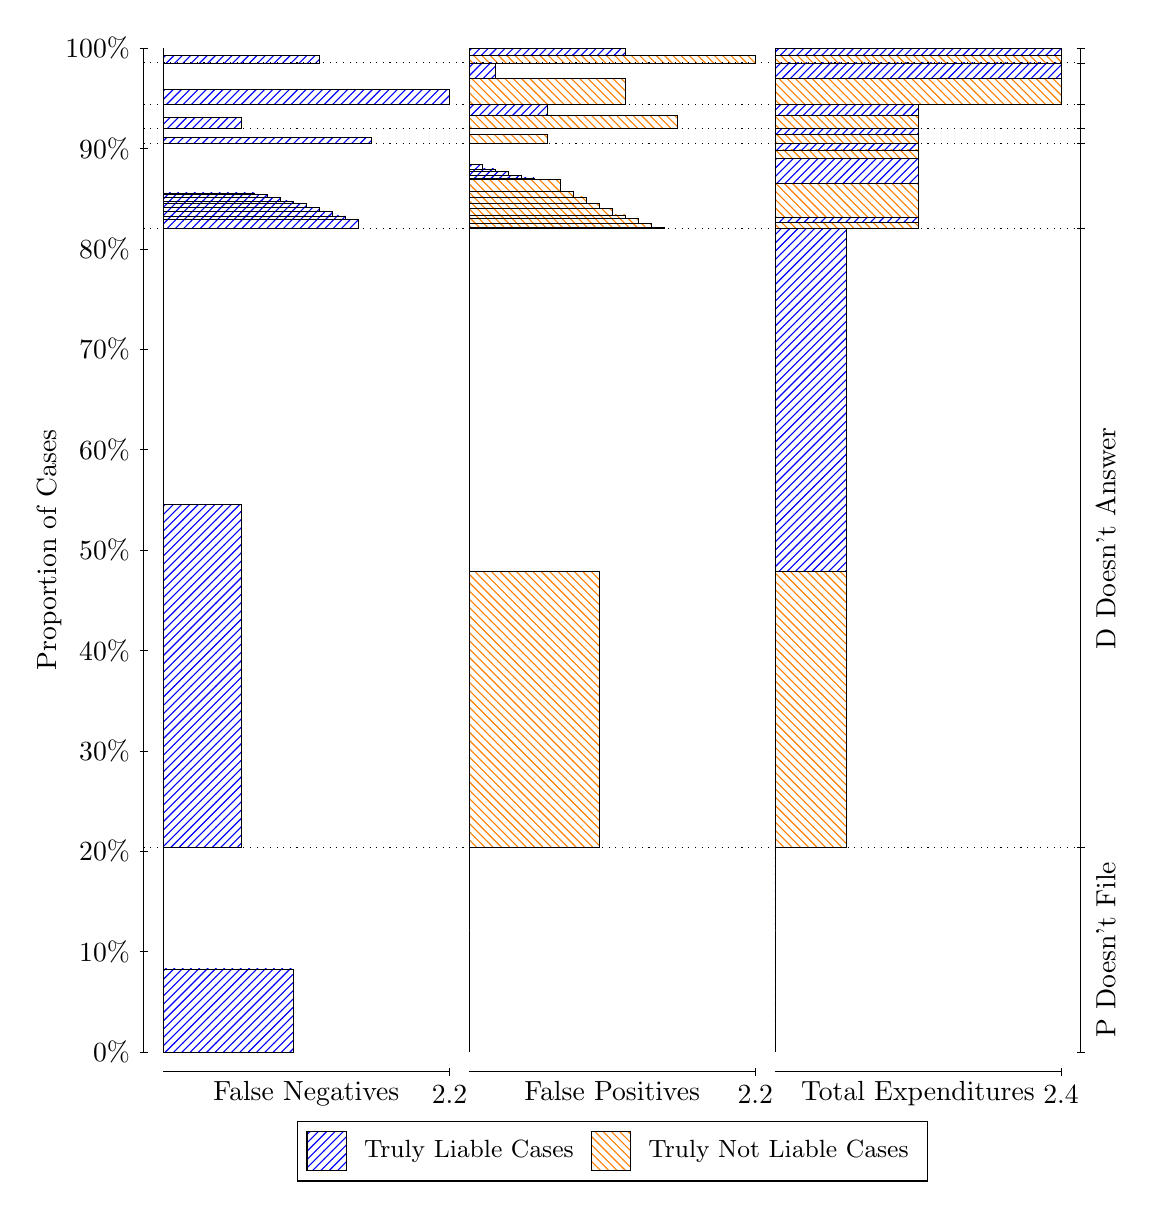
\begin{tikzpicture}
\draw[black, very thin] (1.5,1.75) -- (1.5,14.5);
\node[rotate=90, anchor=center] at (0.3, 8.125) {Proportion of Cases};
\draw[black, very thin] (1.45,1.75) -- (1.55,1.75);
\node[anchor=east] at (1.45, 1.75) {0\%};
\draw[black, very thin] (1.45,3.025) -- (1.55,3.025);
\node[anchor=east] at (1.45, 3.025) {10\%};
\draw[black, very thin] (1.45,4.3) -- (1.55,4.3);
\node[anchor=east] at (1.45, 4.3) {20\%};
\draw[black, very thin] (1.45,5.575) -- (1.55,5.575);
\node[anchor=east] at (1.45, 5.575) {30\%};
\draw[black, very thin] (1.45,6.85) -- (1.55,6.85);
\node[anchor=east] at (1.45, 6.85) {40\%};
\draw[black, very thin] (1.45,8.125) -- (1.55,8.125);
\node[anchor=east] at (1.45, 8.125) {50\%};
\draw[black, very thin] (1.45,9.4) -- (1.55,9.4);
\node[anchor=east] at (1.45, 9.4) {60\%};
\draw[black, very thin] (1.45,10.675) -- (1.55,10.675);
\node[anchor=east] at (1.45, 10.675) {70\%};
\draw[black, very thin] (1.45,11.95) -- (1.55,11.95);
\node[anchor=east] at (1.45, 11.95) {80\%};
\draw[black, very thin] (1.45,13.225) -- (1.55,13.225);
\node[anchor=east] at (1.45, 13.225) {90\%};
\draw[black, very thin] (1.45,14.5) -- (1.55,14.5);
\node[anchor=east] at (1.45, 14.5) {100\%};

\draw[black, very thin] (13.4,1.75) -- (13.4,14.5);
\draw[black, very thin] (13.35,1.75) -- (13.45,1.75);
\node[anchor=west] at (13.35, 1.75) {};
\draw[black, very thin] (13.35,4.3465) -- (13.45,4.3465);
\node[anchor=west] at (13.35, 4.3465) {};
\draw[black, very thin] (13.35,12.205) -- (13.45,12.205);
\node[anchor=west] at (13.35, 12.205) {};
\draw[black, very thin] (13.35,13.289) -- (13.45,13.289);
\node[anchor=west] at (13.35, 13.289) {};
\draw[black, very thin] (13.35,13.482) -- (13.45,13.482);
\node[anchor=west] at (13.35, 13.482) {};
\draw[black, very thin] (13.35,13.781) -- (13.45,13.781);
\node[anchor=west] at (13.35, 13.781) {};
\draw[black, very thin] (13.35,14.311) -- (13.45,14.311);
\node[anchor=west] at (13.35, 14.311) {};
\draw[black, very thin] (13.35,14.5) -- (13.45,14.5);
\node[anchor=west] at (13.35, 14.5) {};

\draw[black, very thin, pattern color=blue, pattern=north east lines] (1.75,1.75) rectangle (3.4015,2.8051);
\draw[black, very thin, pattern color=orange, pattern=north west lines] (1.75,2.8051) rectangle (1.75,4.3465);
\draw[black, very thin, pattern color=blue, pattern=north east lines] (1.75,4.3465) rectangle (2.7409,8.7007);
\draw[black, very thin, pattern color=orange, pattern=north west lines] (1.75,8.7007) rectangle (1.75,12.205);
\draw[black, very thin, pattern color=blue, pattern=north east lines] (1.75,12.205) rectangle (4.2273,12.319);
\draw[black, very thin, pattern color=blue, pattern=north east lines] (1.75,12.319) rectangle (4.0621,12.369);
\draw[black, very thin, pattern color=blue, pattern=north east lines] (1.75,12.369) rectangle (3.897,12.427);
\draw[black, very thin, pattern color=blue, pattern=north east lines] (1.75,12.427) rectangle (3.7318,12.472);
\draw[black, very thin, pattern color=blue, pattern=north east lines] (1.75,12.472) rectangle (3.5667,12.53);
\draw[black, very thin, pattern color=blue, pattern=north east lines] (1.75,12.53) rectangle (3.4015,12.56);
\draw[black, very thin, pattern color=blue, pattern=north east lines] (1.75,12.56) rectangle (3.2364,12.608);
\draw[black, very thin, pattern color=blue, pattern=north east lines] (1.75,12.608) rectangle (3.0712,12.642);
\draw[black, very thin, pattern color=blue, pattern=north east lines] (1.75,12.642) rectangle (2.9061,12.66);
\draw[black, very thin, pattern color=orange, pattern=north west lines] (1.75,12.66) rectangle (1.75,13.289);
\draw[black, very thin, pattern color=blue, pattern=north east lines] (1.75,13.289) rectangle (4.3924,13.366);
\draw[black, very thin, pattern color=orange, pattern=north west lines] (1.75,13.366) rectangle (1.75,13.482);
\draw[black, very thin, pattern color=blue, pattern=north east lines] (1.75,13.482) rectangle (2.7409,13.62);
\draw[black, very thin, pattern color=orange, pattern=north west lines] (1.75,13.62) rectangle (1.75,13.781);
\draw[black, very thin, pattern color=blue, pattern=north east lines] (1.75,13.781) rectangle (5.3833,13.978);
\draw[black, very thin, pattern color=orange, pattern=north west lines] (1.75,13.978) rectangle (1.75,14.311);
\draw[black, very thin, pattern color=blue, pattern=north east lines] (1.75,14.311) rectangle (3.7318,14.409);
\draw[black, very thin, pattern color=orange, pattern=north west lines] (1.75,14.409) rectangle (1.75,14.5);
\draw[black, very thin, pattern color=orange, pattern=north west lines] (5.6333,1.75) rectangle (5.6333,3.2913);
\draw[black, very thin, pattern color=blue, pattern=north east lines] (5.6333,3.2913) rectangle (5.6333,4.3465);
\draw[black, very thin, pattern color=orange, pattern=north west lines] (5.6333,4.3465) rectangle (7.2848,7.8509);
\draw[black, very thin, pattern color=blue, pattern=north east lines] (5.6333,7.8509) rectangle (5.6333,12.205);
\draw[black, very thin, pattern color=orange, pattern=north west lines] (5.6333,12.205) rectangle (8.1106,12.226);
\draw[black, very thin, pattern color=orange, pattern=north west lines] (5.6333,12.226) rectangle (7.9455,12.27);
\draw[black, very thin, pattern color=orange, pattern=north west lines] (5.6333,12.27) rectangle (7.7803,12.335);
\draw[black, very thin, pattern color=orange, pattern=north west lines] (5.6333,12.335) rectangle (7.6152,12.38);
\draw[black, very thin, pattern color=orange, pattern=north west lines] (5.6333,12.38) rectangle (7.45,12.463);
\draw[black, very thin, pattern color=orange, pattern=north west lines] (5.6333,12.463) rectangle (7.2848,12.525);
\draw[black, very thin, pattern color=orange, pattern=north west lines] (5.6333,12.525) rectangle (7.1197,12.61);
\draw[black, very thin, pattern color=orange, pattern=north west lines] (5.6333,12.61) rectangle (6.9545,12.68);
\draw[black, very thin, pattern color=orange, pattern=north west lines] (5.6333,12.68) rectangle (6.7894,12.834);
\draw[black, very thin, pattern color=blue, pattern=north east lines] (5.6333,12.834) rectangle (6.4591,12.852);
\draw[black, very thin, pattern color=blue, pattern=north east lines] (5.6333,12.852) rectangle (6.2939,12.886);
\draw[black, very thin, pattern color=blue, pattern=north east lines] (5.6333,12.886) rectangle (6.1288,12.934);
\draw[black, very thin, pattern color=blue, pattern=north east lines] (5.6333,12.934) rectangle (5.9636,12.964);
\draw[black, very thin, pattern color=blue, pattern=north east lines] (5.6333,12.964) rectangle (5.7985,13.022);
\draw[black, very thin, pattern color=blue, pattern=north east lines] (5.6333,13.022) rectangle (5.6333,13.289);
\draw[black, very thin, pattern color=orange, pattern=north west lines] (5.6333,13.289) rectangle (6.6242,13.405);
\draw[black, very thin, pattern color=blue, pattern=north east lines] (5.6333,13.405) rectangle (5.6333,13.482);
\draw[black, very thin, pattern color=orange, pattern=north west lines] (5.6333,13.482) rectangle (8.2758,13.643);
\draw[black, very thin, pattern color=blue, pattern=north east lines] (5.6333,13.643) rectangle (6.6242,13.781);
\draw[black, very thin, pattern color=orange, pattern=north west lines] (5.6333,13.781) rectangle (7.6152,14.113);
\draw[black, very thin, pattern color=blue, pattern=north east lines] (5.6333,14.113) rectangle (5.9636,14.311);
\draw[black, very thin, pattern color=orange, pattern=north west lines] (5.6333,14.311) rectangle (9.2667,14.402);
\draw[black, very thin, pattern color=blue, pattern=north east lines] (5.6333,14.402) rectangle (7.6152,14.5);
\draw[black, very thin, pattern color=orange, pattern=north west lines] (9.5167,1.75) rectangle (9.5167,3.2913);
\draw[black, very thin, pattern color=blue, pattern=north east lines] (9.5167,3.2913) rectangle (9.5167,4.3465);
\draw[black, very thin, pattern color=orange, pattern=north west lines] (9.5167,4.3465) rectangle (10.425,7.8509);
\draw[black, very thin, pattern color=blue, pattern=north east lines] (9.5167,7.8509) rectangle (10.425,12.205);
\draw[black, very thin, pattern color=orange, pattern=north west lines] (9.5167,12.205) rectangle (11.333,12.288);
\draw[black, very thin, pattern color=blue, pattern=north east lines] (9.5167,12.288) rectangle (11.333,12.347);
\draw[black, very thin, pattern color=orange, pattern=north west lines] (9.5167,12.347) rectangle (11.333,12.784);
\draw[black, very thin, pattern color=blue, pattern=north east lines] (9.5167,12.784) rectangle (11.333,13.098);
\draw[black, very thin, pattern color=orange, pattern=north west lines] (9.5167,13.098) rectangle (11.333,13.206);
\draw[black, very thin, pattern color=blue, pattern=north east lines] (9.5167,13.206) rectangle (11.333,13.289);
\draw[black, very thin, pattern color=orange, pattern=north west lines] (9.5167,13.289) rectangle (11.333,13.405);
\draw[black, very thin, pattern color=blue, pattern=north east lines] (9.5167,13.405) rectangle (11.333,13.482);
\draw[black, very thin, pattern color=orange, pattern=north west lines] (9.5167,13.482) rectangle (11.333,13.643);
\draw[black, very thin, pattern color=blue, pattern=north east lines] (9.5167,13.643) rectangle (11.333,13.781);
\draw[black, very thin, pattern color=orange, pattern=north west lines] (9.5167,13.781) rectangle (13.15,14.113);
\draw[black, very thin, pattern color=blue, pattern=north east lines] (9.5167,14.113) rectangle (13.15,14.311);
\draw[black, very thin, pattern color=orange, pattern=north west lines] (9.5167,14.311) rectangle (13.15,14.402);
\draw[black, very thin, pattern color=blue, pattern=north east lines] (9.5167,14.402) rectangle (13.15,14.5);
\draw[black, dotted] (1.5,4.3465) -- (13.4,4.3465);
\draw[black, dotted] (1.5,12.205) -- (13.4,12.205);
\draw[black, dotted] (1.5,13.289) -- (13.4,13.289);
\draw[black, dotted] (1.5,13.482) -- (13.4,13.482);
\draw[black, dotted] (1.5,13.781) -- (13.4,13.781);
\draw[black, dotted] (1.5,14.311) -- (13.4,14.311);
\draw[black, very thin] (1.75,1.5) -- (5.3833,1.5);
\node[anchor=north] at (3.5667, 1.5) {False Negatives};
\draw[black, very thin] (5.3833,1.45) -- (5.3833,1.55);
\node[anchor=north] at (5.3833, 1.45) {2.2};

\draw[black, very thin] (5.6333,1.5) -- (9.2667,1.5);
\node[anchor=north] at (7.45, 1.5) {False Positives};
\draw[black, very thin] (9.2667,1.45) -- (9.2667,1.55);
\node[anchor=north] at (9.2667, 1.45) {2.2};

\draw[black, very thin] (9.5167,1.5) -- (13.15,1.5);
\node[anchor=north] at (11.333, 1.5) {Total Expenditures};
\draw[black, very thin] (13.15,1.45) -- (13.15,1.55);
\node[anchor=north] at (13.15, 1.45) {2.4};

\node[black, centered, rotate=90] at (13.72, 3.0482) {P Doesn't File};
\node[black, centered, rotate=90] at (13.72, 8.2758) {D Doesn't Answer};






\draw (7.449999999999999,1.5) node[draw=none] (baseCoordinate) {};
\begin{scope}[align=center]
        \matrix[scale=0.5, draw=black, below=0.5cm of baseCoordinate, nodes={draw}, column sep=0.1cm]{
            \node[rectangle, draw, minimum width=0.5cm, minimum height=0.5cm, pattern=north east lines, pattern color=blue] {}; &
            \node[draw=none, font=\small] (B) {Truly Liable Cases}; &
            \node[rectangle, draw, minimum width=0.5cm, minimum height=0.5cm, pattern=north west lines, pattern color=orange] {}; &
            \node[draw=none, font=\small] (B) {Truly Not Liable Cases}; \\
            };
\end{scope}

\end{tikzpicture}
\end{document}